\documentclass[runningheads,a4paper,oribibl]{llncs}

\usepackage[T1]{fontenc}

\usepackage[utf8]{inputenc}
% \usepackage[latin1]{inputenc}
\usepackage{textcomp}
\usepackage{graphicx}    
\usepackage{url}          

\begin{document}

\pagestyle{headings}

\mainmatter

\title{Exploring the differences in performance between gamers and non-gamers when completing everyday tasks viewed from a third person perspective}


\titlerunning{Third-Person Performance Differences Between Gamers and Nongamers}

\author{Arvid Bräne}

\institute{
	Department of Computing Science \\
	Umeå University, Sweden \\
	\email{arvidbrane@gmail.com} 
}

\maketitle


%\begin{abstract}
%	Here goes the actual text of your abstract.
%\end{abstract}

%\begin{itemize}
%	\item What have I done?
%	\item How did I do it?
%	\item What was the result of the study?
%	\item What to take out from this study
%	\item 2
%	\item 3
%\end{itemize}



\section{Introduction}
The text in this will contain the following:
\begin{itemize}
	\item What have I done?
	\item Why did I do it?
	\item The background to the subject
	\item What is new in this study
	\item References to earlier work such as~\cite{schmierbach2011exploring},~\cite{salamin2006benefits} and~\cite{nakamura20103pi}
	\item Description of what third-person view is
\end{itemize}

\begin{description}
   \item[Purpose] To investigate if there is a measurable difference in performance between people whom have played games and people whom have not.
   \item[Motivation] There is a constantly ongoing debate,~\cite{valadez2012just}, about whether playing video games produce negative side-effects or not. My study investigates one of the possible \emph{positive} performance differences, such as few number of errors and low time consumption.
   \item[Contents] A conclusive investigation of if there is a performance difference of playing video games viewed in third-person or not.
   \item[Resources] The study has been completed using a custom-made rig consisting of a camera, video goggles, carbon fiber booms, 3D-printed parts, batteries and cables. References to earlier work will also be used.
\end{description}

Studies in writing have previously shown that most readers do not have any recognition whether a book was written in first- or third-person ~\cite{hagg2012nya}. 






\section{Method}
Studies prior to this one have been done on the differences between gamers and non-gamers, such as~\cite{schmierbach2011exploring}, but none using hardware to simulate the third-person view experienced in games (see Figure~\ref{fig:GTAIV}) in real life. 

In the following section we will demonstrate our method and the tasks needed to concretise credible results.

\subsection{Overview}

This section should also contain the following:
\begin{itemize}
	\item Give an overview/introduction over/to how this study was completed
	\begin{itemize}
		\item What kind of tasks
		\item Rig design
		\item Task design
		\item Performance benchmarking
	\end{itemize}
	\item References to earlier works
	\item Description about things to take into account
	\item Explaining the form every participant has to fill in
\end{itemize}







\subsection{Survey Design}

This section will describe the function and the design of the survey that the test subjects need to fill in prior to the experiment. The survey should include questions about:
\begin{itemize}
	\item Name
	\item Age
	\item Gender
	\item Hours per week spent playing games
	\item How many years the have been playing games
	\item If the subject considers itself a gamer or not
	\item What types of games the subject plays
\end{itemize}











\subsection{Task Design}
In order for to get the required measurements with high credibility the tasks performed by the test subjects needed to be carefully planed, prepared and executed. To get as wide spread results as possible a few different types of tasks had to be completed by the test subjects:

\begin{description}
   \item[Ball Control Test] The test subject rolls a ball and hits a target in order for it to successfully complete the task. Number of tries required will be noted.
   \item[Balance Test] The test subject will have to walk on a thin straight line placed flat on the ground for as far or as long as it can. Number of seconds and distance will be noted.
   \item[Precision Test] The test subject walks forward facing thorough a preplanned course on flat ground marked with cones as fast and precise as possible. This task is then repeated, but backwards facing. Number of errors and time will be noted
   \item[Task 4] \emph{Might add one or two more...}
\end{description}











\subsection{Rig Design}
In order to see the difference in performance a rig was constructed to produce a game-like third person view, see Figure~\ref{fig:GTAIV}. The test-rig consists of three major parts:
\begin{enumerate}
	\item \textbf{Video Camera}: Constantly recording the test subject and generating a live stream.
	\item \textbf{Mount}: Which the camera is mounted upon in order to get the correct angle.
	\item \textbf{Video Goggles}: Covering the test subjects eyes so he/she cannot see anything other than the live video stream from the camera
\end{enumerate}
The final result of what the rig looks like when put together correctly can be found in Figure~\ref{fig:RigDesign}.

\begin{figure}
   \centering
   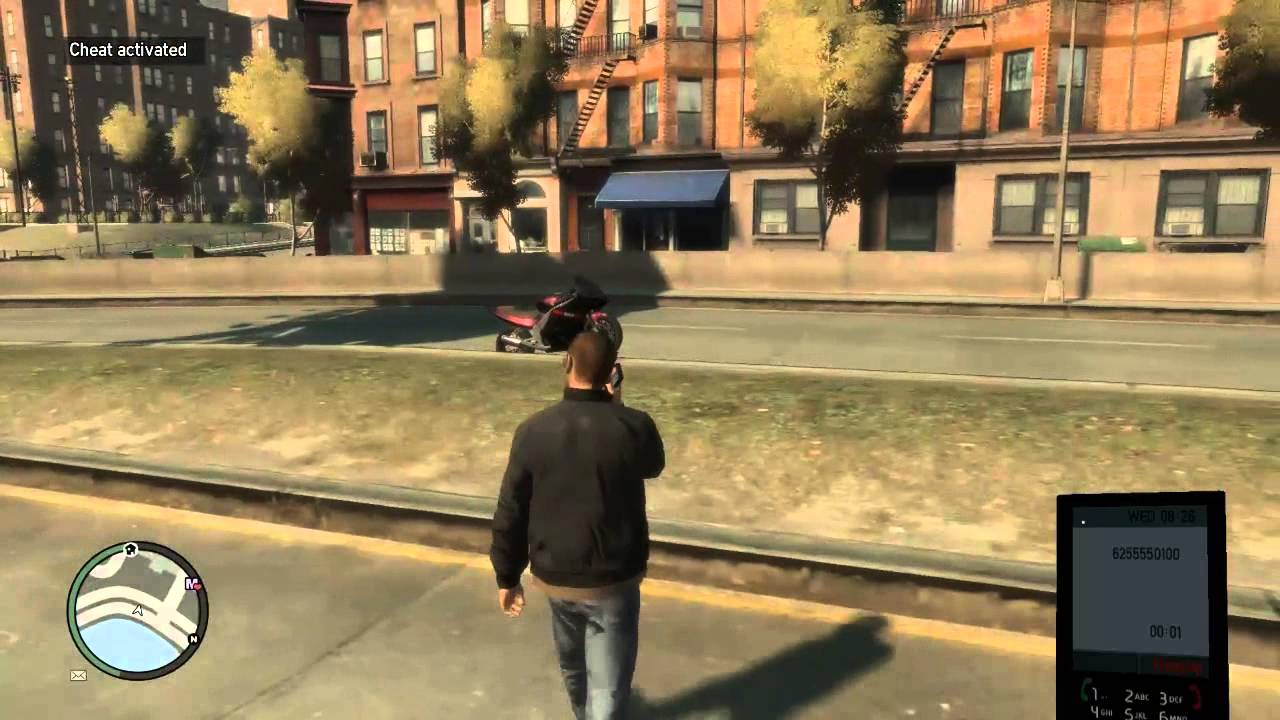
\includegraphics[width=\textwidth]{GTA}
   \caption{A typical third-person view in the game \emph{Grand Theft Auto: IV}. \label{fig:GTAIV}}
\end{figure}

\begin{figure}
   \centering
   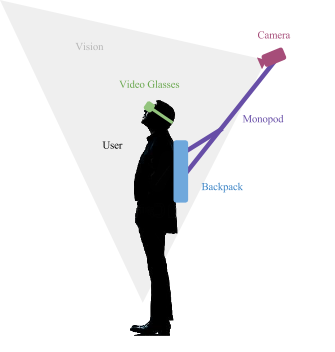
\includegraphics[width=0.5\textwidth]{Rig}
   \caption{A detailed overview of different parts of the rig. \label{fig:RigDesign}}
\end{figure}



\subsection{Interviews}

This section will consist of why and what types of interview questions the test subjects will be asked afterwards. These questions might, or might not, include the following:
\begin{itemize}
	\item What was hard?
	\item What was easy?
	\item Did it feel like you were in a video game?
\end{itemize}







\section{Results}
This section will cover the results from the tests that where done and;
\begin{itemize}
	\item The results from the tests
	\item Diagrams comparing the results
	\item Results of earlier work
	\item Compare the performance between the different groups
\end{itemize}





\section{Discussion}
A general discussion about the study such as:
\begin{itemize}
	\item What part/conclusion in my study could be biast/not reliable
	\item What does my results mean?
	\item Earlier work, how do they compare to my work and what does that mean?
	\item References to earlier work such as~\cite{schmierbach2011exploring}
\end{itemize}



\subsection{Limitations and Drawbacks}
Due to the time and budget limit there are several ways to improve upon my study, ways of doing this might include:
\begin{itemize}
	\item Building a more rigid rig.
	\item Using a more comprehensive camera mounted on a stabilized gimbal.
	\item Using more sophisticated video goggles, such as the Oculus Rift.
\end{itemize}




\subsection{Conclusion}
As a finish, and a complement to the abstract, the conclusion should contain:
\begin{itemize}
	\item What to take out from the study
	\item How this study can be made more in-depth
	\item Future work
\end{itemize}





\nocite{*}
\bibliographystyle{splncs}
% \bibliographystyle{plain-annote}

\bibliography{Bibliography}


\end{document}